%
% This is the LaTeX template file for lecture notes for EE 382C/EE 361C.
%
% To familiarize yourself with this template, the body contains
% some examples of its use.  Look them over.  Then you can
% run LaTeX on this file.  After you have LaTeXed this file then
% you can look over the result either by printing it out with
% dvips or using xdvi.
%
% This template is based on the template for Prof. Sinclair's CS 270.

\documentclass[twoside]{article}
\usepackage{graphicx}
\usepackage{listings}
\lstset
{ %Formatting for code in appendix
    language=Matlab,
    basicstyle=\footnotesize,
    numbers=left,
    xleftmargin=1cm,
    stepnumber=1,
    showstringspaces=false,
    tabsize=1,
    breaklines=true,
    breakatwhitespace=false,
}

\graphicspath{ {images/} }
\setlength{\oddsidemargin}{0.25 in}
\setlength{\evensidemargin}{-0.25 in}
\setlength{\topmargin}{-0.6 in}
\setlength{\textwidth}{6.5 in}
\setlength{\textheight}{8.5 in}
\setlength{\headsep}{0.75 in}
\setlength{\parindent}{0 in}
\setlength{\parskip}{0.1 in}

%
% The following commands set up the lecnum (lecture number)
% counter and make various numbering schemes work relative
% to the lecture number.
%
\newcounter{lecnum}
\renewcommand{\thepage}{\thelecnum-\arabic{page}}
\renewcommand{\thesection}{\thelecnum.\arabic{section}}
\renewcommand{\theequation}{\thelecnum.\arabic{equation}}
\renewcommand{\thefigure}{\thelecnum.\arabic{figure}}
\renewcommand{\thetable}{\thelecnum.\arabic{table}}

%
% The following macro is used to generate the header.
%
\newcommand{\lecture}[4]{
   \pagestyle{myheadings}
   \thispagestyle{plain}
   \newpage
   \setcounter{lecnum}{#1}
   \setcounter{page}{1}
   \noindent
   \begin{center}
   \framebox{
      \vbox{\vspace{2mm}
    \hbox to 6.28in { {\bf EE 382V: Parallel Algorithms
                        \hfill Summer 2017} }
       \vspace{4mm}
       \hbox to 6.28in { {\Large \hfill Lecture #1: #2  \hfill} }
       \vspace{2mm}
       \hbox to 6.28in { {\it Lecturer: #3 \hfill Scribe: #4} }
      \vspace{2mm}}
   }
   \end{center}
   \markboth{Lecture #1: #2}{Lecture #1: #2}
   %{\bf Disclaimer}: {\it These notes have not been subjected to the
   %usual scrutiny reserved for formal publications.  They may be distributed
   %outside this class only with the permission of the Instructor.}
   \vspace*{4mm}
}

%
% Convention for citations is authors' initials followed by the year.
% For example, to cite a paper by Leighton and Maggs you would type
% \cite{LM89}, and to cite a paper by Strassen you would type \cite{S69}.
% (To avoid bibliography problems, for now we redefine the \cite command.)
% Also commands that create a suitable format for the reference list.
\renewcommand{\cite}[1]{[#1]}
\def\beginrefs{\begin{list}%
        {[\arabic{equation}]}{\usecounter{equation}
         \setlength{\leftmargin}{2.0truecm}\setlength{\labelsep}{0.4truecm}%
         \setlength{\labelwidth}{1.6truecm}}}
\def\endrefs{\end{list}}
\def\bibentry#1{\item[\hbox{[#1]}]}

%Use this command for a figure; it puts a figure in wherever you want it.
%usage: \fig{NUMBER}{SPACE-IN-INCHES}{CAPTION}
\newcommand{\fig}[3]{
			\vspace{#2}
			\begin{center}
			Figure \thelecnum.#1:~#3
			\end{center}
	}
% Use these for theorems, lemmas, proofs, etc.
\newtheorem{theorem}{Theorem}[lecnum]
\newtheorem{lemma}[theorem]{Lemma}
\newtheorem{proposition}[theorem]{Proposition}
\newtheorem{claim}[theorem]{Claim}
\newtheorem{corollary}[theorem]{Corollary}
\newtheorem{definition}[theorem]{Definition}
\newenvironment{proof}{{\bf Proof:}}{\hfill\rule{2mm}{2mm}}

% **** IF YOU WANT TO DEFINE ADDITIONAL MACROS FOR YOURSELF, PUT THEM HERE:

\begin{document}
%FILL IN THE RIGHT INFO.
%\lecture{**LECTURE-NUMBER**}{**DATE**}{**LECTURER**}{**SCRIBE**}
\lecture{22}{July 23}{Vijay Garg}{Brice Ngnigha}
%\footnotetext{These notes are partially based on those of Nigel Mansell.}

% **** YOUR NOTES GO HERE:

% Some general latex examples and examples making use of the
% macros follow.  
%**** IN GENERAL, BE BRIEF. LONG SCRIBE NOTES, NO MATTER HOW WELL WRITTEN,
%**** ARE NEVER READ BY ANYBODY.
\section{Introduction}
In this lecture, we will build on our previous lecture on the Euler Tour technique to solve problems such as rooting a tree, computing a vertex level, and computing the number of descendants of a tree.

\section{Rooting a Tree}
Given a tree T = (V, E) rooted at a node r. For every node v $\neq$ r, we want to find the parent of v, P(v) when the tree T is rooted at r.

Considering the trees below, we compute the root of each vertex:

\begin{figure}[!h]
\centering
\begin{minipage}{.5\textwidth}
  \centering
  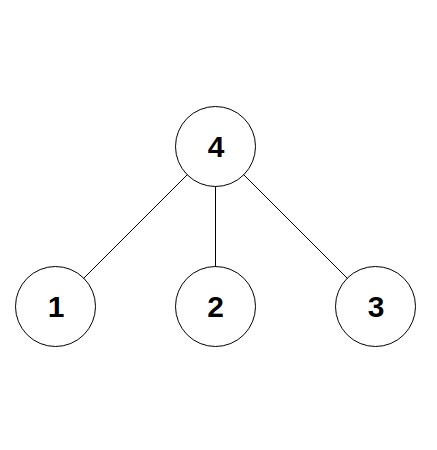
\includegraphics[scale=.25]{g1}
  \caption{Tree rooted at 4} $P(1) = 4\hspace{0.5cm}P(2) = 4\hspace{0.5cm}P(3) = 4\hspace{0.5cm}P(1) = \emptyset$
  \label{fig:test1}
\end{minipage}%
\begin{minipage}{.5\textwidth}
  \centering
  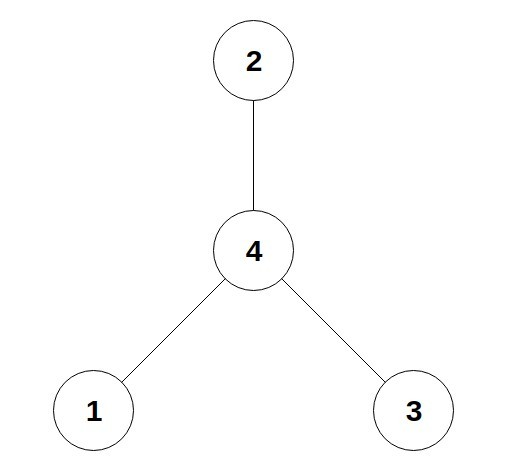
\includegraphics[scale=.25]{g2}
  \caption{Tree rooted at 2} $P(1) = 4\hspace{0.5cm}P(1) = 4\hspace{0.5cm}P(3) = 4\hspace{0.5cm}P(2) = \emptyset$
  \label{fig:test2}
\end{minipage}
\end{figure}

\subsection{Algorithm}
$Input: $ A tree T(Given as adjacency list), a node r, the root of T.\\
$Output: $ For every vertex v $\neq$ r, the parent P(v).\\

\begin{enumerate}
\item Convert the Euler Circuit into the Euler Path
\item Set $succ(u_{d-1}, r)$ to $null$
\item Assign wieght w = 1to each edge in the linked list\\
Apply parallel prefix on the linked list
\item For each edge (x, y) in parallel do \\
if prefsum(x,y) < prefsum(y,x) then P(y) = x
\end{enumerate}

\subsection{Example}
Tree rooted at node 2:\\
\begin{center}
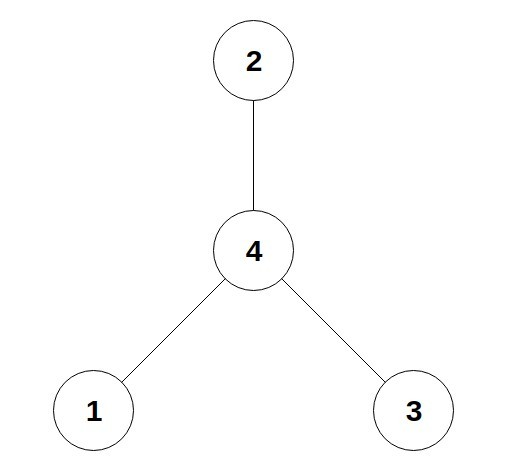
\includegraphics[scale=0.25]{g2} \\
Euler Circuit : $(1,4)\to(4,2)\to(2,4)\to(4,3)\to(3,4)\to(4,1)\to\to\to\to(1,4)$
\end{center}

\begin{center}
 \begin{tabular}{||c c||} 
 \hline
    Operation & Result \\
 \hline
 	Euler Path & $(2,4)\to(4,3)\to(3,4)\to(4,1)\to(1,4)\to(4,2)$ \\ 
 \hline
 	Weight w & $(1)\to(1)\to(1)\to(1)\to(1)\to(1)$ \\
 \hline
 	PrefixSum & $(1)\to(2)\to(3)\to(4)\to(5)\to(6)$ \\
 \hline
\end{tabular}
\end{center}

\section{Computing the Vertex Level}
Given a tree T = (V, E) rooted at a node r. For every node v $\neq$ r, we want to find the level of v, which is the number of edges from vertex v to the root r.

Considering the tree below, we compute the level of each vertex:

\begin{figure}[!h]
\centering
\begin{minipage}{.5\textwidth}
  \centering
  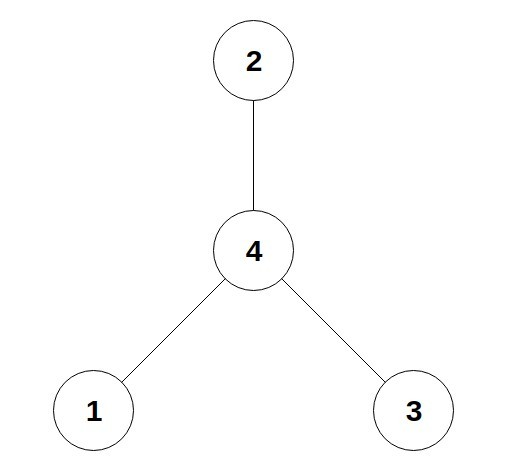
\includegraphics[scale=.25]{g2}
  \caption{Tree rooted at 1} 
  $level(2) = 0\hspace{0.5cm}level(4) = 1\hspace{0.5cm}level(1) = 2 \hspace{0.5cm}level(3) = 2$
  \label{fig:test1}
\end{minipage}%
\end{figure}

\subsection{Algorithm}
\paragraph{•}
$Input: $ A tree T(Given as adjacency list), a node r, the root of T.
$Input: $ For every vertex v $\neq$ r,output level(v), the distance from vertex v to the root.

\begin{enumerate}
\item Compute Euler Path for the rooted tree r
\item For all v ≠ r do in par \\
      w (p(v), v) = -1 ; w(v, p(v)) = -1
\item Perform prefix – sum 
\item For each v ≠ r do in par \\
      level(v) = prefix sum (p(), v)
\item level(r) = 0
\end{enumerate}

\subsection{Example}

\begin{figure}[!h]
\centering
\begin{minipage}{.5\textwidth}
  \centering
  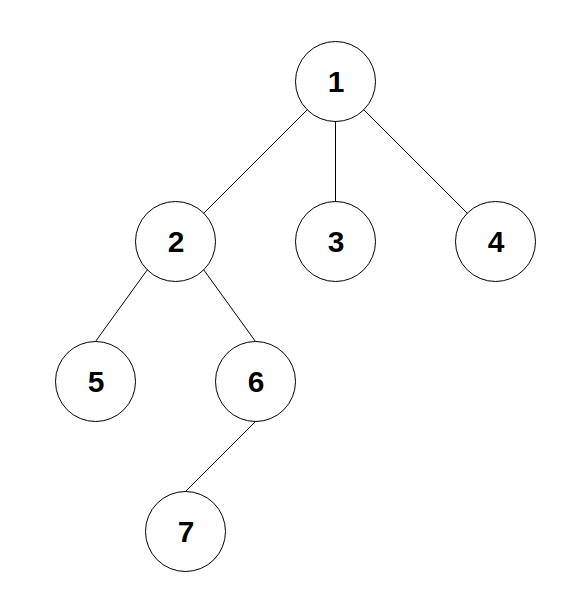
\includegraphics[scale=.3]{g3}
  \caption{Tree rooted at 1} 
  \label{fig:test1}
\end{minipage}%
\centering
\begin{minipage}{.5\textwidth}
  \centering
  \begin{center}
  \begin{tabular}{||c c c||} 
  \hline
     Euler Peth & Weights & Prefix Sum \\
  \hline
     (1,2) & {+1} & {1} \\
  \hline
  	 (2,5) & {+1} & {2} \\
  \hline
 	 (5,2) & {-1} & {1} \\
  \hline
 	 (2,6) & {+1} & {2} \\
  \hline
 	 (6,7) & {+1} & {3} \\
  \hline
 	 (7,6) & {-1} & {2} \\
  \hline
 	 (6,2) & {-1} & {1} \\
  \hline
 	 (2,1) & {-1} & {0} \\
  \hline
 	 (1,3) & {+1} & {1} \\
  \hline
 	 (3,1) & {-1} & {0} \\
  \hline
 	 (1,4) & {+1} & {1} \\
  \hline
 	 (4,1) & {-1} & {0} \\
  \hline
  \end{tabular}
  \end{center}
  \caption{some cap}
\label{fig:test1}
\end{minipage}%
\end{figure}

\subsection{result}
\begin{figure} [!h]
\centering
\begin{minipage}{.5\textwidth}
  \centering
  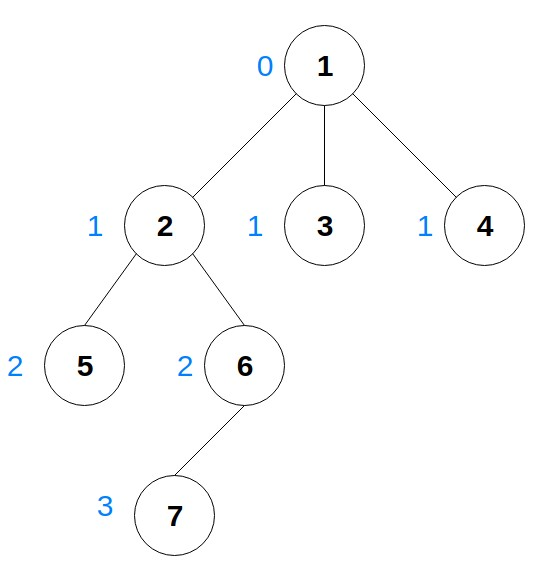
\includegraphics[scale=.3]{g4}
  \caption{Tree with node level.} 
  \label{fig:test1}
\end{minipage}%
\end{figure}


\section{Computing the Number of Descendants}
Given a tree T = (V, E) rooted at a node r. For every node v $\neq$ r, we want to find the parent of v, P(v) when the tree T is rooted at r.

Considering the trees below, we compute the root of each vertex:

\begin{figure}[!h]
\centering
\begin{minipage}{.5\textwidth}
  \centering
  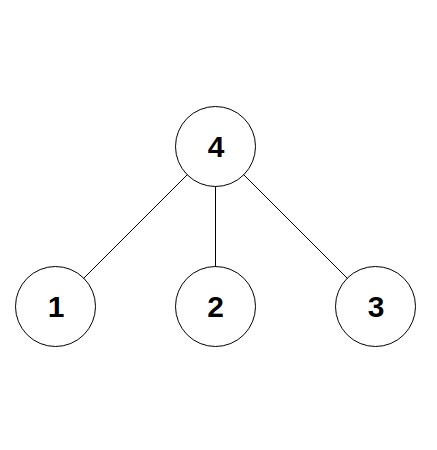
\includegraphics[scale=.25]{g1}
  \caption{Tree rooted at 4} $P(1) = 4\hspace{0.5cm}P(2) = 4\hspace{0.5cm}P(3) = 4\hspace{0.5cm}P(1) = \emptyset$
  \label{fig:test1}
\end{minipage}%
\begin{minipage}{.5\textwidth}
  \centering
  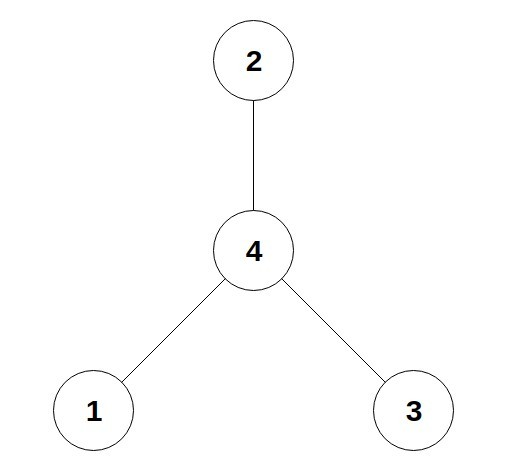
\includegraphics[scale=.25]{g2}
  \caption{Tree rooted at 2} $P(1) = 4\hspace{0.5cm}P(1) = 4\hspace{0.5cm}P(3) = 4\hspace{0.5cm}P(2) = \emptyset$
  \label{fig:test2}
\end{minipage}
\end{figure}

\subsection{Algorithm}
$Input: $ A tree T(Given as adjacency list), a node r, the root of T.
$Input: $ For every vertex v $\neq$ r, the parent P(v).

\begin{enumerate}
\item Convert the Euler Circuit into the Euler Path
\item Set $succ(u_{d-1}, r)$ to $null$
\item Assign wieght w = 1to each edge in the linked list\\
Apply parallel prefix on the linked list
\item For each edge (x, y) in parallel do \\
\indent if prefsum(x,y) < prefsum(y,x) then P(y) = x \\
\end{enumerate}

\subsection{Example}
Tree rooted at node 2:\\
\begin{center}
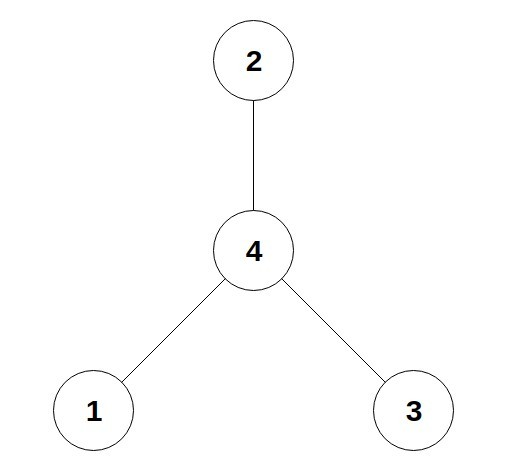
\includegraphics[scale=0.25]{g2} \\
Euler Circuit : $(1,4)\to(4,2)\to(2,4)\to(4,3)\to(3,4)\to(4,1)\to\to\to\to(1,4)$
\end{center}

\begin{center}
 \begin{tabular}{||c c||} 
 \hline
    Operation & Result \\
 \hline
 	Euler Path & $(2,4)\to(4,3)\to(3,4)\to(4,1)\to(1,4)\to(4,2)$ \\ 
 \hline
 	Weight w & $(1)\to(1)\to(1)\to(1)\to(1)\to(1)$ \\
 \hline
 	PrefixSum & $(1)\to(2)\to(3)\to(4)\to(5)\to(6)$ \\
 \hline
\end{tabular}
\end{center}

\end{document}







